Since a signficant portion of this thesis uses the performance of 
CBC searches as a metric for the quality of the 
data, a more thorough discussion of how a CBC search 
works is necessary. This thesis will focus on the output of the PyCBC 
pipeline, which is a Python-based software packaged used to search for 
gravitational waves \cite{Usman:2015kfa,pycbc-github}

CBC search pipelines are designed to search for gravitational wave transients 
from compact binary coalescences \cite{Usman:2015kfa}. 
The signals expected to be measured in the LIGO interferometers are extremely quiet, 
with gravitational wave strains on the order of $10^{-22}$. On these scales, most 
signals will not be able to be extracted from the background noise with simple filtering. 
Figure \ref{fig:quiet-BNS} shows the gravitational wave strain from a 1.4-1.4$M_{\odot}$ 
binary neutron star system at a distance of 20 Mpc overlaid on real detector noise from 
the Livingston 
interferometer. The signal has a peak strain roughly two orders of magnitude lower than 
the peak strain of the detector noise. 
For this reason, the CBC searches employ a matched filter algorithm, which correlates 
expected CBC
waveforms with detector data and assigns a ranking statistic, the signal-to-noise 
ratio (SNR), to every event that it finds. 

\subsection{The matched filter}

The matched filter calculates the correlation of the detector data with expected CBC 
waveforms in the frequency domain. The detector data and expected waveform are 
multiplied together and their product is divided by the background noise in the detector. 
The fundamental operation of the matched filter is defined as an inner product of the 
detector data and the CBC waveform \cite{Usman2015:kfa},
\begin{equation}
(s|h)(t) = 4\mathrm{Re}\int_{f_\mathrm{low}}^{f_\mathrm{high}} \frac{\tilde{s}(f)\tilde{h}^*(f)}{S_n (f)}e^{2\pi i f t}\, \mathrm{d}f,
\label{eq:inner-product}
\end{equation}
where $\tilde{s}$ is the Fourier transformed detector data, $\tilde{h}$ is the Fourier
transformed gravitational waveform, and $S_n (f)$ is the power spectral
density of the detector data averaged over 2048 seconds, which represents the average 
noise in the detector. The bounds of the integral are set to span the frequency space 
for which the interferometers are sensitive enough to detect gravitational waves, 
typically 30 - 2000 Hz. 

As described in Equation \ref{eq:strain}, a gravitational wave is comprised of two 
polarizations, ``h-plus" and ``h-cross". When the data are searched for a CBC  
signal, a waveform is generated for each polarization and the matched filter is 
computed separately for each polarization. 
The SNR of a CBC waveform at any given time is defined as the weighted quadrature sum 
of the SNR measured for each polarization \cite{Usman:kfa}, 
\begin{equation}
\rho^2(t) = \frac{(s|h_\mathrm{p})^2 + (s|h_\mathrm{c})^2}{(h_\mathrm{p}|h_\mathrm{p})},
\label{eq:snr}
\end{equation}
where $h_\mathrm{p}$ and $h_\mathrm{c}$ are the plus and cross polarizations of the 
modeled gravitational waveform respectively and $s$ is the detector data. 
When the SNR time-series defined in equation \ref{eq:snr} crosses a certain threshold, 
the waveform is considered to have significant overlap with the detector data and an 
event is generated at the time of the SNR peak. These events are called ``triggers'' 
and are used to generate populations of potential gravitational wave events for analysis.

\begin{figure}[ht!]
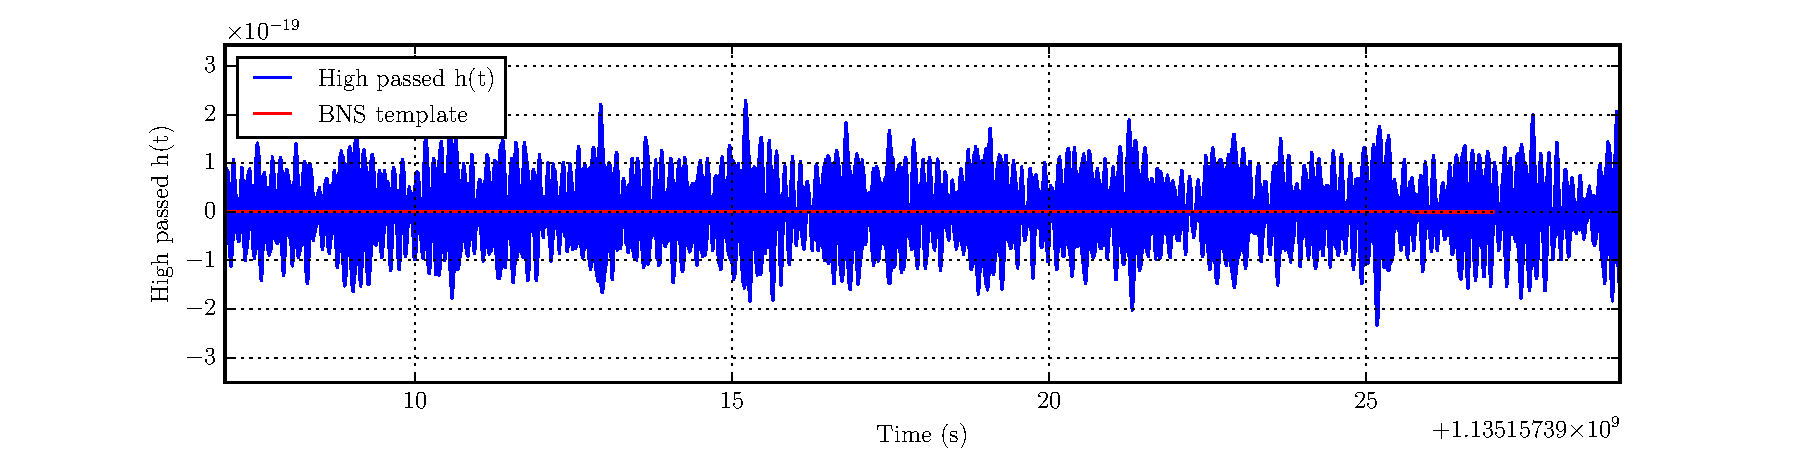
\includegraphics[width=\textwidth]{figures/introduction/quiet_BNS}
\caption[BNS signal in detector noise]{A simulated gravitational wave signal from a %
         binary neutron star system overlaid on real detector noise from L1. %
         The blue curve, labeled $h(t)$, represents the detector data. %
         The red curve represents %
         the gravitational wave strain expected from a 1.4-1.4$M_{\odot}$ %
         binary neutron star system %
         at 20 Mpc. The peak strain of the binary neturon star waveform is %
         $8\times10^{-22}$. %
         The detector data have been high pass filtered with a corner frequency %
         at 20 Hz and show a peak strain of $2.2\times10^{-19}$. The signal is %
         buried in the detector noise and requires a matched filter algorithm %
         to be recovered. At this time, the inspiral range for a 1.4-1.4$M_{\odot}$ %
         BNS system was 60 Mpc, indicating that the same system originating at 60 Mpc %
         would be recovered with SNR = 8. % 
         }
\label{fig:quiet-BNS}
\end{figure}

\subsection{Waveform templates}

To perform a search, the matched filter algorithm needs to know what to search for.
A collection of expected CBC waveforms is generated using
the formalism of general relativity before the analysis \cite{Pan:2009wj,Purrer:2015tud}.
Each of the expected waveforms is called a template and
the full collection of waveforms is referred to as the template bank. This template bank
is constructed to span the astrophysical parameter space included in the search
\cite{GW150914-CBC}. This parameter space is constrained by the noise spectrum of 
the interferometers. As shown in Figure \ref{fig:noise-budget}, the LIGO 
interferometers are sensitive enough to detect gravitational waves in the 
region from roughly 30 - 2000 Hz. This rules out detection of sources that are expected to 
coalesce at very low frequencies, such as supermassive black hole binaries 
\cite{Merloni:2008tj} and 
binary white dwarf systems \cite{PostnovYungelson:2006}. 
The template bank used in Advanced LIGO's first observing 
run consisted waveforms representing binary neutron stars, binary black holes, 
and neutron star-black hole binary systems \cite{GW150914-CBc}. 
The total masses of these systems ranged from 
2-100$M_{\odot}$. This reflects the set of systems that will have merger frequencies 
above 30 Hz and will have detectable power in LIGO's sensitive bandwidth.

Each waveform is defined by the mass and spin of each compact
object in the binary system. 
It is convenient to combine
the component masses into a new variable, chirp mass, which is used to
parameterize gravitational wave signals in general relativity. Chirp mass is defined
as
\begin{equation}
M_{chirp} = \frac{(m_1m_2)^{3/5}}{(m_1 + m_2)^{1/5}}
\end{equation}
where the $m_{i}$ are the component masses of the compact objects in the
binary system. 
It is also convenient to combine the effects of each
object's spin into one parameter called effective spin, $\chi_{eff}$,
which is the
mass-weighted spin of the system \cite{Privitera:2013xza}. $\chi_{eff}$ is defined as
\begin{equation}
\chi_{eff} = \frac{\chi_{1}m_{1} + \chi_{2}m_{2}}{m_{1} + m_{2}}
\end{equation}
where the $\chi_{i}$ are the dimensionless spin parameters \cite{Kidder:1995zr}
and the $m_{i}$ are the masses for each compact object in the binary system. 

\subsection{$\chi^{2}$ signal consistency test}\label{sec:chisq}

If the data produced by the interferometers were Gaussian, the matched filter would 
be sufficient for running a search pipeline and recovering gravitational wave signals. 
Unfortunately, the data are non-Gaussian, containing noise transients of varying 
durations \cite{Nuttall:2015dqa,GW150914-DETCHAR}. These noise transients, 
or ``glitches", can have significant amplitude 
and, when multiplied with a waveform template in the matched filter, can cause 
loud triggers to be generated. 
However, a significant advantage of performaing a modeled search for gravitational 
waves is that 
we know we're looking for. With this information, the SNR can be refined into a more 
robust ranking statistic for significant events in the data. This is done using the 
$\chi^{2}$ signal consistency test \cite{Allen:2004gu}. 

The SNR produced by the matched filter is an integral in the frequency domain which 
reports the total accumulated SNR over a given bandwidth. If a noise transient has 
significant amplitude, it can generate a high SNR trigger by overlapping with the 
waveform template in the matched filter. However, these noise 
transients typically have a duration on the order of 0.1s. This type of transient 
is easily distinguished from a chirp signal that increases monotonically in frequency 
over the span of many seconds. 
The $\chi^{2}$ test divides each CBC waveform into
frequency bins of equal power, checking that the SNR is distributed as a 
function of frequency
as expected from an actual CBC signal.
For a signal divided into $p$ frequency bins, each bin should contain $\frac{1}{p}$ of the power in the 
signal. 
In the $\chi^2$ calculation, the SNR is calculated for each frequency bin and compared to the expected 
amount. The $\chi^2$ statistic is calculated as \cite{Usman:2015kfa}
\begin{equation}
\chi^2 = p\displaystyle\sum_{l=1}^{p}\left[\left(\frac{\rho_\mathrm{p}^2}{p}-\rho_{\mathrm{p},l}^2\right)^2 + \left(\frac{\rho^2_\mathrm{c}}{p}-\rho_{\mathrm{c},l}^2\right)^2 \right] \, ,
\label{eq:chisqr}
\end{equation}
where $\rho^2_\mathrm{p}$ is the SNR of the plus polarization of the waveform, $\rho^2_\mathrm{c}$ 
is the SNR of the cross 
polarization of the waveform, $p$ is the number of frequency bins, and 
$\rho^2_{i,l}$ is the calculated SNR for the $l^\mathrm{th}$ frequency bin.
The $\chi^2$ statistic is then normalized such that a real signal will be reported with a value of 1. 
This normalized $\chi^2$ is called the reduced $\chi^2$ and is denoted by $\chi^2_r$.

In the PyCBC search, each trigger that comes out of the matched filter search is 
weighted based on the results of
the $\chi^{2}$ test. This is folded into a new ranking statistic for CBC triggers,
which is called re-weighted SNR and is denoted by $\hat{\rho}$.
The re-weighted SNR is calculated as \cite{Usman:2015kfa} 
\begin{equation}
\hat{\rho} = \left\{\begin{array}{lr}
\rho\left/\left[(1+(\chi^2_r)^3)/2\right]^\frac{1}{6}\right., & \text{if } \chi_r^2 > 1, \\
\rho, & \text{if } \chi_r^2 \le 1,
\label{eq:reweighted}
\end{array}\right.
\end{equation}
where $\rho$ is the measured SNR and $\chi^2_r$ is the reduced $\chi^2$.
It is important to note that if a real signal has a power
distribution that matches the template waveform, it will not be
down-weighted by the $\chi^{2}$ test.  

This test is extremely powerful, as shown in Figure \ref{fig:cbc-newsnr-histograms}, 
which shows the distribution of single detector PyCBC triggers generated from 
September 12 to October 20, 2015. 
Figure \ref{subfig:l1-snr-hist} shows the distribution of triggers in SNR. 
The extensive tail of
triggers with high SNR, which is generated when high amplitude noise transients 
are processed by the matched filter, extends beyond SNR 100. 
These high SNR triggers are down-weighted in the re-weighted SNR distribution,
leaving behind a tail that extends to $\hat{\rho} \approx$ 11.5 as seen in Figure 
\ref{subfig:l1-newsnr-hist}. Keeping in mind that a real signal will be reported 
at the same value in each plot, the re-weighting of triggers has lowered the 
noise floor, allowing for signals with SNR $>$ 11.5 to stand out as the 
loudest events in their respective interferometers rather than being buried 
beneath a population of high SNR triggers.  

\begin{figure}[!ht]%
\centering
  \subfloat[]{
      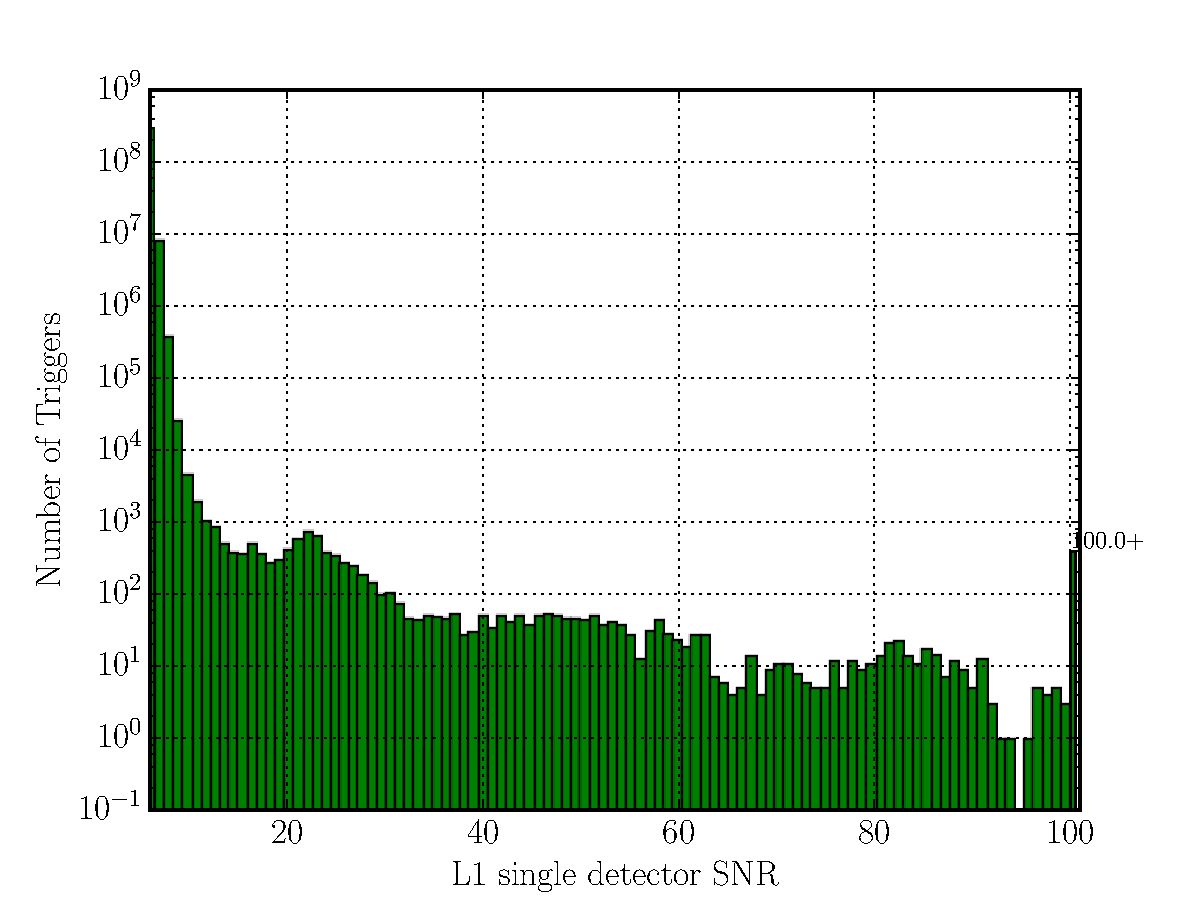
\includegraphics[width=.75\textwidth]{figures/introduction/l1-snr-histogram}
      \label{subfig:l1-snr-hist}
  }

  \subfloat[]{
      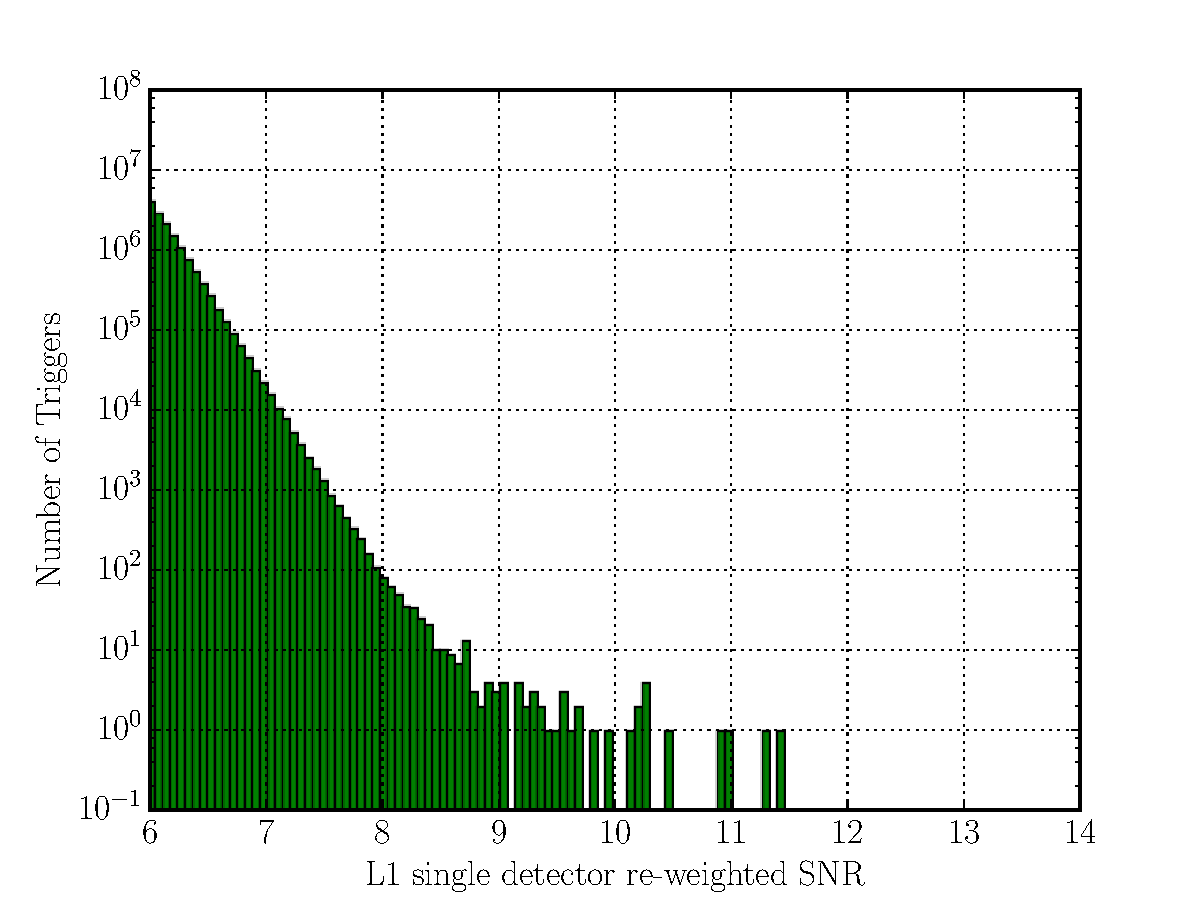
\includegraphics[width=.75\textwidth]{figures/introduction/l1-newsnr-histogram}
      \label{subfig:l1-newsnr-hist}
  }

  \caption[PyCBC SNR and re-weighted SNR histograms]{Histograms of single interferometer PyCBC %
           triggers from the Livingston (L1) interferometer. %
           These triggers were generated from September 12 to October 20, 2015. These histograms %
           contain triggers from the entire template bank, but %
           exclude any triggers found in coincidence between the two interferometers. %
           (\ref{subfig:l1-snr-hist}) A histogram of single interferometer triggers in SNR. %
           The tail of this distribution extends beyond SNR = 100. %
           (\ref{subfig:l1-newsnr-hist}) A histogram of single interferometer triggers in re-weighted SNR. %
           The chi-squared test down-weights the long tail of SNR triggers %
           in the re-weighted SNR distribution. Note that the x-axis has different %
           limits in each plot.}
  \label{fig:cbc-newsnr-histograms}
\end{figure}

The remaining tail of re-weighted SNR triggers represents the loudest 
background triggers in the CBC search. Investigating this set of
loudest background triggers guides data quality efforts in defining the current 
limiting noise sources to the CBC search. This process is detailed in Chapter 
\ref{ch:instrumentalDetchar}.

\subsection{Searching for signals}

The matched filter algorithm is run separately on each interferometer's data using the 
same bank 
of template waveforms. The output of the matched filter, the SNR time-series, is scanned 
for peaks and a set of single interferometer 
triggers is generated. The two sets of single interferometer triggers are then compared to
search for any events that were recorded within 15ms of each other.
Gravitational waves are predicted by general relativity to travel
at the speed of light. The light travel time between the two interferometers is 10 ms
and 5ms is added to the coincidence window due to uncertainty in signal arrival time
\cite{GW150914-CBC}.
As such, any triggers that are found within 15 ms of each other and
are recovered with the same source parameters are considered to be coincident between 
the two
interferometers. These coincident triggers represent potential gravitational wave signals
and are referred to as ``foreground events". 

The ranking statistic for coincident events in the PyCBC search is the network
re-weighted SNR, $\hat{\rho}_{c}$, which is the quadrature sum of the re-weighted
SNR from each interferometer.  
\begin{equation}
\hat{\rho}_{c} = \sqrt{\hat{\rho}^2_L + \hat{\rho}^2_H}
\end{equation}
where $\hat{\rho}_L$ is the re-weighted SNR measured in the Livingston detector 
and $\hat{\rho}_H$ is the re-weighted SNR measured in the Hanford detector.

Most of these foreground events will be
chance coincidences between noise in each interferometer, which is expected given
the number of events in each data set. A large number of foreground events will be 
generated due to the detector noise, but ideally the distribution of foreground events 
will fall of sharply in $\hat{\rho}_{c}$, allowing for genuine signals to be 
recognized. To understand how stastically significant a foreground event is, a background 
distribution must be generated.

To generate the background distribution, we return to the set of single interferometer 
triggers that were generated when the matched filter was initially run. Since we want 
to understand the distribution of triggers based on detector noise, all of the triggers 
that were found to be coincident between the two interferometers are removed from the 
data sets, effectively removing all
potential gravitational wave signals. The remaining triggers are then due to fluctuations 
in the background noise in each interferometer. These two sets of triggers,
one from each interferometer, are then time shifted by a duration longer than the
light travel time between the interferometers.
Since gravitational waves are predicted to travel at the speed of light,
this time shift ensures that the
two sets of triggers are astrophysically uncorrelated and do not contain any gravitational
wave signals. The coincidence test is then performed again with the time shifted triggers,
resulting in a coincident trigger set which represents background noise. 
A full distribution of background triggers is generated by performing this timeslide
technique every 0.1 seconds and iterating over all of the data used in the search 
\cite{Usman2015:kfa}. This 
distribution tells us how often we should expect to see coincident triggers with the 
same waveform parameters at a given value of SNR.

The statistical significance of any candidate gravitational wave is
evaluated by calculating the rate of background events from detector noise 
that are at least as
loud as the candidate event \cite{GW150914-CBC}. 
The results of the first observing run and details on 
the significance of foreground events is presented in Chapter \ref{ch:o1results}. 
Any loud triggers that appear as the result of instrumental
transients will contribute to the tail of the background distribution and
the influence the statistical significance of a recovered foreground event.
The process of performing data quality investigations and data validation are 
detailed in Chapter \ref{ch:instrumentalDetchar}

\subsection{Gating}\label{sec:gating}

The PyCBC search includes a data conditioning stage that applies preventative  
cuts to remove large transients from the input data stream. 
This is done in a process called gating \cite{Usman:2015kfa}, which uses a
window function to remove times containing large transients from the input data stream. This is done
by applying a smooth windowing function to the problematic section of data, excising the large transient.
The gating process is tuned by modifying the selection criteria for transients to be removed and
by adjusting the time window to remove around each transient.
Chapters \ref{ch:GW150914-DQ} and \ref{ch:GW151226-DQ} contain details about the 
gating thresholds used for the analyses containing GW150914 and GW151226 respectively. 

